%%% License: Creative Commons Attribution Share Alike 4.0 (see https://creativecommons.org/licenses/by-sa/4.0/)
%%% Slides are based heavily on earlier versions of this course taught by Jesper Rudiger.

\documentclass[english,10pt
%,handout
,aspectratio=169
]{beamer}
%%% License: Creative Commons Attribution Share Alike 4.0 (see https://creativecommons.org/licenses/by-sa/4.0/)
%%% Slides are based heavily on earlier versions of this course taught by Jesper Rudiger and Peter Norman Sorensen.

\DeclareGraphicsExtensions{.eps, .pdf,.png,.jpg,.mps,}
\usetheme{reMedian}
\usepackage{parskip}
\makeatother

\renewcommand{\baselinestretch}{1.1} 

\usepackage{amsmath, amssymb, amsfonts, amsthm}
\usepackage{enumerate}
\usepackage{hyperref}
\usepackage{url}
\usepackage{bbm}
\usepackage{color}

\usepackage{tikz}
\usepackage{tikzscale}
\newcommand*\circled[1]{\tikz[baseline=(char.base)]{
		\node[shape=circle,draw, inner sep=-20pt] (char) {#1};}}
\usetikzlibrary{automata,positioning}
\usetikzlibrary{decorations.pathreplacing}
\usepackage{pgfplots}
\usepgfplotslibrary{fillbetween}
\usepackage{graphicx}

\usepackage{setspace}
%\thinmuskip=1mu
%\medmuskip=1mu 
%\thickmuskip=1mu 


\usecolortheme{default}
\usepackage{verbatim}
\usepackage[normalem]{ulem}

\usepackage{apptools}
\AtAppendix{
	\setbeamertemplate{frame numbering}[none]
}
\usepackage{natbib}




\title{Financial Markets Microstructure \\ Exercise class 2}

\author{Egor Starkov}

\date{K{\o}benhavns Unversitet \\
	Spring 2020}



\begin{document}
	\AtBeginSection[]{
		\frame<beamer>{
			\frametitle{This lecture:}
			\tableofcontents[currentsection,currentsubsection]
	}}
%\frame[plain]{\titlepage}
\addtocounter{framenumber}{-1}



\section{Glosten-Milgrom model}

\begin{frame}{Lecture 3}
	\begin{itemize}
		\item FPR chapter 3 exercises (p. 124-125):
		\begin{itemize}
			%\item exercise 2 -- solve GM model with numbers instead of letters
			\item exercise 3 about the GM model where speculators are not perfectly informed, but instead receive a signal about the value of the asset
		\end{itemize}
		\item Bonus problem: GM model with uniform $v$
	\end{itemize}
\end{frame}




%\subsection{ex 2}
%
%\begin{frame}{Exercise 2}
%	A small risky company's stock is worth either \$10 ($v_L$) or \$20 ($v_H$) with probability 1/2 each ($\theta=1-\theta=1/2$).
%	\begin{enumerate}[a]
%		\small 
%		\item Compute  bid and ask prices set by risk neural competitive market makers in the absence of informed trading.
%		\item Compute bid and ask prices set by risk neutral competitive market makers when they expect 1/10 of trade initiators to be informed (know the stock's true value) and to trade as profit maximizers, while the other 9/10 are uninformed and buy or sell with \textit{equal probability}. Assume  all transactions are the same size.
%		\item Compute the average trading cost to an uninformed trader and the average gain to an informed one, assuming a unit trade size in both cases.
%		\item Do you agree with the following statement? ``Insider trading does not harm most market participants: it harms only those who are unlucky enough to trade with an insider.''
%	\end{enumerate}
%\end{frame}
%
%
%\begin{frame}{Exercise 2.a}
%	\begin{exampleblock}{}
%		(a) Compute  bid and ask prices set by risk neural competitive market makers in the absence of informed trading.
%	\end{exampleblock}
%	
%	\begin{align*}
%		a &= \mathbb{E}[v | \Omega, Buy]
%		\\
%		\visible<2->{
%			&= \frac{\frac{1}{2} \beta_B 20 + \frac{1}{2} \beta_B 10}{\frac{1}{2} \beta_B + \frac{1}{2} \beta_B} = 15
%		}
%	\end{align*}
%	\begin{align*}
%		b &= \mathbb{E}[v | \Omega, Sell]
%		\\
%		\visible<2->{
%			&= \frac{\frac{1}{2} \beta_B 20 + \frac{1}{2} \beta_B 10}{\frac{1}{2} \beta_B + \frac{1}{2} \beta_B} = 15
%		}
%	\end{align*}
%\end{frame}
%
%
%\begin{frame}{Exercise 2.b}
%	\begin{exampleblock}{}
%		(b) Compute bid and ask prices set by risk neutral competitive market makers when they expect 1/10 of trade initiators to be informed (know the stock's true value) and to trade as profit maximizers, while the other 9/10 are uninformed and buy or sell with equal probability. Assume  all transactions are the same size.
%	\end{exampleblock}
%	\vspace{-1em}
%	\begin{align*}
%		a &= \mathbb{E}[v | \Omega, Buy]
%		\\
%		\visible<2->{
%			&= \frac{\frac{1}{2} \left(0.1 + 0.9\cdot\frac{1}{2}\right) 20 + \frac{1}{2} \left(0.9 \cdot \frac{1}{2}\right) 10}{\frac{1}{2} \left(0.1 + 0.9\cdot\frac{1}{2}\right) + \frac{1}{2} \left(0.9 \cdot \frac{1}{2}\right)} = 15.5
%		}
%	\end{align*}
%	\begin{align*}
%		b &= \mathbb{E}[v | \Omega, Sell]
%		\\
%		\visible<2->{
%			&= \frac{\frac{1}{2} \left(0.9 \cdot \frac{1}{2}\right) 20 + \frac{1}{2} \left(0.9\cdot\frac{1}{2} + 0.1\right) 10}{\frac{1}{2} \left(0.9 \cdot \frac{1}{2}\right) + \frac{1}{2} \left(0.9\cdot\frac{1}{2} + 0.1\right)} = 14.5
%		}
%	\end{align*}
%\end{frame}
%
%
%\begin{frame}{Exercise 2.c}
%	\begin{exampleblock}{}
%		(c) Compute the average trading cost to an uninformed trader and the average gain to an informed one, assuming a unit trade size in both cases.
%	\end{exampleblock}
%	\pause
%	\begin{align*}
%		\mathbb{E} \Pi_U = \frac{1}{2} (15-15.5) + \frac{1}{2} (14.5-15) = -0.5
%	\end{align*}
%	\begin{align*}
%		\mathbb{E} \Pi_I = \frac{1}{2} (20 - 15.5) + \frac{1}{2} (14.5 - 10) = 4.5
%	\end{align*}
%	(note that $\frac{1}{2}-\frac{1}{2}$ probabilities relate to different events in the two expressions)
%\end{frame}
%
%
%\begin{frame}{Exercise 2.d}
%	\begin{exampleblock}{}
%		(d) Do you agree with the following statement? 
%		\begin{quotation}
%			\smallskip
%			``Insider trading does not harm most market participants: it harms only those who are unlucky enough to trade with an insider.''
%		\end{quotation}
%	\end{exampleblock}
%	\pause
%	No. Uninformed traders pay the cost arising from informed trading, even if they do not trade directly with the informed traders.
%\end{frame}




\subsection{ex 3}

\begin{frame}{Exercise 3}
	\begin{itemize}
		\item $v \in \{v^H,v^L\}$ w.p. $\frac{1}{2}$;
		\item dealer competitive, risk-neutral, does not know $v$;
		\item trader uninformed w.p. $1-\pi$, then buys and sells w.p. $\frac{1}{2}$;
		\item trader informed w.p. $\pi$, then observes \structure{signal about state}
		\begin{itemize}
			\item signal accurate w.p. $\rho \in \left(\frac{1}{2},1\right]$.
		\end{itemize}
	\end{itemize}
\end{frame}


\begin{frame}{Exercise 3.a}
	\begin{exampleblock}{}
		(a) Write dealer's expected profits upon receiving buy/sell order, assuming informed trader follows his signal.
	\end{exampleblock}
	\begin{align*}
		\mathbb{E} [\Pi_D | Buy] &= 
		\visible<2->{
			\frac{ \pi \frac{1}{2} \rho (a-v^H) + \pi \frac{1}{2} (1-\rho) (a-v^L) + (1-\pi) \frac{1}{2} (a-\mu)}{\pi \frac{1}{2} \rho + \pi \frac{1}{2} (1-\rho) + (1-\pi) \frac{1}{2} }
			\\
			&= \pi \rho (a - v^H) + \pi (1-\rho) (a-v^L) + (1-\pi) (a - \mu)
		}
	\end{align*}
	\begin{align*}
		\mathbb{E} [\Pi_D | Sell] &= 
		\visible<2->{
			\frac{ \pi \frac{1}{2} \rho (v^L-b) + \pi \frac{1}{2} (1-\rho) (v^H-b) + (1-\pi) \frac{1}{2} (\mu-b)}{\pi \frac{1}{2} \rho + \pi \frac{1}{2} (1-\rho) + (1-\pi) \frac{1}{2} }
			\\
			&= \pi \rho (v^L-b) + \pi (1-\rho) (v^H-b) + (1-\pi) (\mu - b)
		}
	\end{align*}
	\visible<2->{where $\mu = \frac{v^H+v^L}{2}$.}
\end{frame}


\begin{frame}{Exercise 3.b}
	\begin{exampleblock}{}
		(b) Compute the bid and ask prices set by a risk-neutral competitive dealer.
	\end{exampleblock}
	\begin{align*}
		a &= 
		\visible<2->{\pi \rho v^H + \pi (1-\rho) v^L + (1-\pi) \mu
		}
	\end{align*}
	\begin{align*}
		b &= 
		\visible<2->{\pi \rho v^L + \pi (1-\rho) v^H + (1-\pi) \mu
		}
	\end{align*}
	\visible<2->{from $\mathbb{E} [\Pi_D | Buy] = \mathbb{E} [\Pi_D | Sell] = 0$.}
\end{frame}


\begin{frame}{Exercise 3.c}
	\begin{exampleblock}{}
		(c) Derive bid-ask spread as a function of signal's informativeness $\rho$. When is the market more or less liquid? Why?
	\end{exampleblock}
	\begin{align*}
		S &= a - b
		\\
		\visible<2->{
			&= \pi (2\rho - 1) (v^H - v^L)
		}
	\end{align*}
	\visible<2->{Higher $\rho$ $\Leftrightarrow$ larger $S$ $\Leftrightarrow$ less liquid market because of larger adverse selection costs (same as larger $\pi$).}
\end{frame}


\begin{frame}{Exercise 3.d}
	\begin{exampleblock}{}
		(d) Verify that the speculator's strategy (buy after signal $H$, sell after signal $L$) is optimal.
	\end{exampleblock}
	Consider signal $H$:
	\begin{align*}
		\mathbb{E} [\Pi_I | H, Buy] &= 
		\visible<2->{
			\rho (v^H - a) + (1-\rho) (v^L - a)
			\\
			&= \left( \rho v^H + (1-\rho) v^L - \mu \right) (1-\pi) > 0
		}
	\end{align*}
	\begin{align*}
		\mathbb{E} [\Pi_I | H, Sell] &= 
		\visible<2->{
			\rho (b - v^H) + (1-\rho) (b - v^L)
			\\
			&= (1-\pi) \left[ \mu - (\rho v^H + (1-\rho) v^L) \right] - \pi (2\rho - 1) (v^H - v^L) < 0
		}
	\end{align*}
	\visible<2->{Same for signal $L$.}
\end{frame}




\subsection{GM with Uniform value}

\begin{frame}{GM with Uniform value}
	\begin{itemize}
		\item \textbf{Uniform outcome}: Suppose $v$ is uniformly distributed on [0,1]
		\item \textbf{Prior value}: Prior density $f(v) = 1$, and $\mu = \mathbb{E}[v] = \int_0^1 v f(v) dv= 1/2$
		\item Look for an ask price $a < 1$:
		\begin{itemize}
			\item Speculator buys if  $v>a$ and sells if $v<b$ ($v=a$ has zero prob.). Thus:
			\begin{equation*}
			\mathbb{P}(Buy|v) = 
			\left\{
			\begin{aligned}
			(1-\pi) \beta_B + \pi 	&\text{ if } v > a; \\
			(1-\pi) \beta_B 		&\text{ if } v<a.
			\end{aligned}
			\right.
			\end{equation*}
			\item Recall Bayes' Rule: $f(v|  Buy) = \frac{f(v) \mathbb{P}(Buy| v)} {\mathbb{P}(Buy)}$. Then,
			\begin{equation*}
			f(v|  Buy)=\left\{
			\begin{aligned}
			&\frac{(1-\pi)\beta_B + \pi} {(1-\pi)\beta_B + (1-a)\pi}	&& \text{ if } v>a; \\
			&\frac{(1-\pi)\beta_B} {(1-\pi)\beta_B + (1-a)\pi}		&& \text{ if } v<a.
			\end{aligned}
			\right.
			\end{equation*}
		\end{itemize}
	\end{itemize}
\end{frame}


\begin{frame}{GM with Uniform value (2)}
	Now we explicity have $a$ on both sides of $a=\mathbb{E}[v|Buy]$. Must solve:
	\begin{align*}
	a 
	& = \mathbb{E}[v|Buy] \\
	& = \int^{a}_0 \frac{(1-\pi) \beta_B \cdot \structure{v}}{(1-\pi)\beta_B + (1-a) \pi} \, dv + \int^{1}_{a} \frac{[(1-\pi) \beta_B + \pi] \cdot \alert{v}}{(1-\pi)\beta_B + (1-a) \pi} \, dv \\
	& =  \frac{(1-\pi) \beta_B \cdot \structure{a^2/2}}{(1-\pi)\beta_B + (1-a) \pi}+  \frac{[(1-\pi) \beta_B + \pi] \cdot \alert{(1-a^2)/2}}{(1-\pi)\beta_B + (1-a) \pi} \\
	& =  \frac{(1-\pi) \beta_B + \pi -\pi a^2}{2(1-\pi)\beta_B + 2(1-a) \pi} = \frac{1}{2} + \frac{\pi a (1 - a)}{2(1-\pi)\beta_B + 2(1-a) \pi}
	\end{align*}
	This is a quadratic equation in $a$. For $\pi=\beta_B=1/2$, solution is $a=\frac{3}{2} \pm \frac{\sqrt{3}}{2}$. Since we assumed $a<1$, equilibrium in this case  is $a=\frac{3}{2} - \frac{\sqrt{3}}{2}$.
\end{frame}



%
%\section{Trading costs and Inventory risk}
%\subsection{ex 9}
%
%\begin{frame}{Lecture 4}
%	\begin{itemize}
%		\item If you are bored, solve \hyperlink{ex9}{Exercise 9} on page 128 about the bid-ask spread in the mean-SD model
%		\item If you feel like a challenge, solve \hyperlink{ex10}{Exercise 10} on page 128
%	\end{itemize}
%\end{frame}
%
%
%\begin{frame}[label=ex9]{Exercise 9}
%	\begin{itemize}
%		\item Two-period model with inventory risk;
%		\item dealer's utility: $U = \mathbb{E}_t [w_{t+1}] - \rho \sqrt{\mathbb{V}(w_{t+1})}$;
%		\item dealer can receive a buy order $y_t > 0$ or sell order $-y_t < 0$ (here $y_t$ is some fixed amount);
%		\item dealer has initial endowment $z_t$.
%	\end{itemize}
%\end{frame}
%
%
%\begin{frame}{Exercise 9.a}
%	\begin{exampleblock}{}
%		(a) Compute the bid-ask spread as a function of $y_t$ when the dealer has a long initial position ($z_t > 0$)
%	\end{exampleblock}
%	\pause
%	\begin{itemize}
%		\item From lecture: the dealer's optimal supply is
%		\begin{itemize}
%			\item Supply any $y_t \leq z_t$ if $p_t = \mu_t - \rho\sigma_{\epsilon}$,
%			\item Supply any $y_t \geq z_t$ if $p_t = \mu_t + \rho\sigma_{\epsilon}$
%		\end{itemize}
%		\item I.e., the ask price is
%		\begin{align*}
%			a_t = 
%			\begin{cases}
%				\mu_t - \rho\sigma_{\epsilon} & \text{ if } y_t \leq z_t;
%				\\
%				\mu_t + \rho\sigma_{\epsilon} & \text{ if } y_t \geq z_t;
%			\end{cases}
%		\end{align*}
%		and the bid price is $b_t = \mu_t - \rho\sigma_{\epsilon}$ for any $y_t$.
%	\end{itemize}
%\end{frame}
%
%
%\begin{frame}{Exercise 9.a}
%	\begin{exampleblock}{}
%		(a) Compute the bid-ask spread as a function of $y_t$ when the dealer has a long initial position ($z_t > 0$)
%	\end{exampleblock}
%	\begin{itemize}
%		\item So spread is
%		\begin{align*}
%			S_t = 
%			\begin{cases}
%				0 & \text{ if } y_t \leq z_t;
%				\\
%				2\rho\sigma_{\epsilon} & \text{ if } y_t \geq z_t;
%			\end{cases}
%		\end{align*}
%	\end{itemize}
%\end{frame}
%
%
%\begin{frame}{Exercise 9.b}
%\begin{exampleblock}{}
%	(b) Compute the bid-ask spread as a function of $y_t$ when the dealer has a short initial position ($z_t < 0$)
%\end{exampleblock}
%\begin{itemize}
%	\item Similar to above:
%	\begin{align*}
%		S_t = 
%		\begin{cases}
%		0 & \text{ if } y_t \leq |z_t|;
%		\\
%		2\rho\sigma_{\epsilon} & \text{ if } y_t \geq |z_t|;
%		\end{cases}
%	\end{align*}
%\end{itemize}
%\end{frame}
%
%
%\begin{frame}{Exercise 9.c}
%	\begin{exampleblock}{}
%		(c) Represent these two cases graphically
%	\end{exampleblock}
%	\centering
%	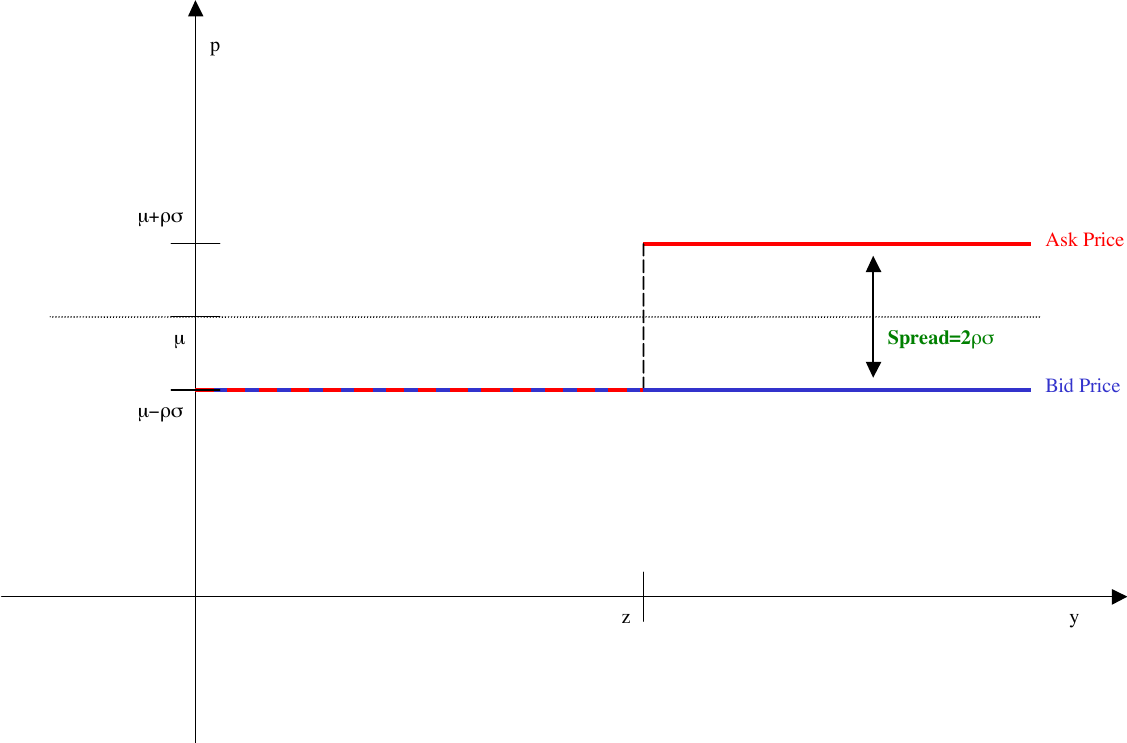
\includegraphics[scale=0.2]{pics/ex9c_1}
%	
%	Case 1: $z_t > 0$
%\end{frame}
%
%
%\begin{frame}{Exercise 9.c}
%	\begin{exampleblock}{}
%		(c) Represent these two cases graphically
%	\end{exampleblock}
%	\centering
%	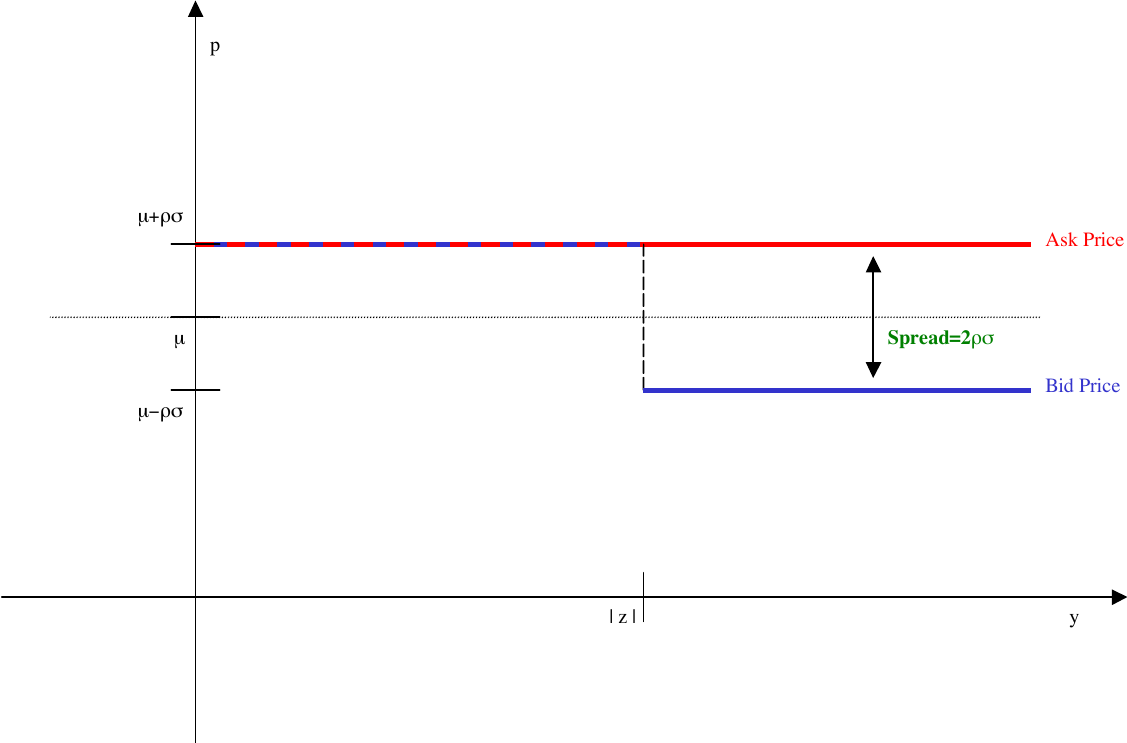
\includegraphics[scale=0.2]{pics/ex9c_2}
%	
%	Case 2: $z_t < 0$
%\end{frame}
%
%
%
%
%\subsection{ex 10}
%
%\begin{frame}[label=ex10]{Exercise 10: inventory cost and order flow risk}
%	\begin{itemize}
%		\item Take inventory cost model from lecture;
%		\item dealer's utility: $\mathbb{E}U(w_{t+1}) = \mathbb{E}_t [w_{t+1}] - \rho \sqrt{\mathbb{V}(w_{t+1})}$;
%		\item dealers competitive and short-sighted (i.e., $\mathbb{E}U(w_{t+1})=0$);
%		\item dealer sets pricing schedule $p_t(y_t)$ depending on order flow $y_t$;
%		\item traders submit single-unit orders ($d_t = \pm 1$):
%		\begin{itemize}
%			\item w.p. $1-\delta$ trader unsophisticated -- places buy/sell order w.p. $1/2$ each;
%			\item w.p. $\delta$ trader price-sensitive -- buys if $p_{t-1} < \mu_{t-1}$, sells if $p_{t-1} > \mu_{t-1}$
%			% idea: traders do not observe p_t, base their decisions around previous period's values
%			\item (no privately informed traders)
%		\end{itemize}
%	\end{itemize}
%\end{frame}
%
%
%\begin{frame}{Exercise 10.a}
%	\begin{exampleblock}{}
%		(a) Assume $p_t = \mu_t - \beta(z_t - y_t) = \mu_t - \beta z_{t+1}$. 
%		
%		Compute $\mathbb{E}_t[p_{t+1}]$ and $\mathbb{V}_t(p_{t+1})$.
%	\end{exampleblock}
%	\pause
%	\begin{itemize}
%		\item Market clearing: $d_t = y_t$;
%		\begin{itemize}
%			\item so if $z_{t+1} > 0$ then $p_t < \mu_t$ then $\mathbb{E}d_{t+1} = \delta$;
%			\item if $z_{t+1} < 0$ then $p_t > \mu_t$ then $\mathbb{E}d_{t+1} = -\delta$.
%		\end{itemize}
%		\item Price at $t+1$ is $p_{t+1} = \mu_{t+1} - \beta(z_{t+1} - d_{t+1})$, so
%		% Expectation computed as of the end of period t, after trades at t -- then z_{t+1} is already known
%		\begin{align*}
%			\mathbb{E}_t [p_{t+1}] &= \mu_t - \beta z_{t+1} + \beta \mathbb{E} [d_{t+1}] = 
%			\begin{cases}
%				\mu_t - \beta z_{t+1} + \beta \delta & \text{ for } z_{t+1} > 0;
%				\\
%				\mu_t & \text{ for } z_{t+1} = 0;
%				\\
%				\mu_t - \beta z_{t+1} - \beta \delta & \text{ for } z_{t+1} < 0;
%			\end{cases}
%			\\
%			\mathbb{V}_t (p_{t+1}) &= 
%			\begin{cases}
%				\beta^2 (1-\delta^2) + \sigma_\epsilon^2 & \text{ for } z_{t+1} \neq 0;
%				\\
%				\beta^2 + \sigma_\epsilon^2 & \text{ for } z_{t+1} = 0;
%			\end{cases}
%		\end{align*}
%	\end{itemize}
%\end{frame}
%
%
%\begin{frame}{Exercise 10.b}
%	\begin{exampleblock}{}
%		(b) Solve for the equilibrium pricing policy.
%	\end{exampleblock}
%	\vspace{-2.5em}
%	\begin{align*}
%		U(y_t) = \mathbb{E}_t [p_{t+1}] (z_t - y_t) + c_t + p_t y_t - \rho \sqrt{\mathbb{V}(p_{t+1})} \cdot | z_t - y_t |
%		% first three elements: Ew_{t+1}, namely current cash ct, revenue from today's sales pt*yt, and expected liquidation cost of remaining holdings
%	\end{align*}
%	Dealer chooses how much to sell given some fixed price $p_t$, so schedule $p_t(y_t)$ must satisfy $\frac{\partial U}{\partial y_t} = 0$. Inverse supply function is then given by:
%	\pause
%	\vspace{-1em}
%	\begin{align*}
%		p_t &= 
%		\begin{cases}
%			\mathbb{E}_t [p_{t+1}] - \rho \sqrt{\mathbb{V}(p_{t+1})} & \text{ if } z_{t+1} > 0
%			\\
%			\mathbb{E}_t [p_{t+1}] & \text{ if } z_{t+1} = 0
%			\\
%			\mathbb{E}_t [p_{t+1}] + \rho \sqrt{\mathbb{V}(p_{t+1})} & \text{ if } z_{t+1} > 0
%		\end{cases}
%		\\
%		&= 
%		\begin{cases}
%		\mu_t - \beta z_{t+1} + \beta \delta - \rho \sqrt{\beta^2 (1-\delta^2) + \sigma_\epsilon^2} & \text{ if } z_{t+1} > 0
%		\\
%		\mu_t & \text{ if } z_{t+1} = 0
%		\\
%		\mu_t - \beta z_{t+1} - \beta \delta + \rho \sqrt{\beta^2 (1-\delta^2) + \sigma_\epsilon^2} & \text{ if } z_{t+1} > 0
%		\end{cases}
%	\end{align*}
%\end{frame}
%
%
%\begin{frame}{Exercise 10.c}
%	\begin{exampleblock}{}
%		(c) Find $\beta$.
%	\end{exampleblock}
%	
%	\pause
%	\begin{itemize}
%		\item We assumed that $p_t = \mu_t - \beta z_{t+1}$.
%		\item For this to coincide with our answer to (b), it must be that 
%		$$ \beta \delta - \rho \sqrt{\beta^2 (1-\delta^2) + \sigma_\epsilon^2} = 0 $$
%		$$ \Leftrightarrow \beta = \frac{\rho \sigma_\epsilon}{\sqrt{\delta^2 - \rho^2(1-\delta^2)}} $$
%		(need $\rho < \sqrt{\frac{\delta^2}{1 - \delta^2}}$)
%		\item $\beta$ increasing in $\rho$ and $\sigma_\epsilon$ -- similar to lecture
%		\item (NEW!) $\beta$ decreasing in $\delta$ -- high $\delta$ means order flow is very predictable, less risk for the dealer. Also $\delta$-traders help dealer rebalance his inventory.
%	\end{itemize}
%\end{frame}
%
%
%\begin{frame}{Exercise 10.d}
%	\begin{exampleblock}{}
%		(d) Compute spread.
%	\end{exampleblock}
%	
%	\pause
%	\begin{itemize}
%		\item We have $p_t(z_{t+1}) = \mu_t - \beta z_{t+1}$, hence
%		\begin{itemize}
%			\item $a_t = p_t(z_t - 1) = \mu_t - \beta z_t + \beta$
%			\item $b_t = p_t(z_t + 1) = \mu_t - \beta z_t - \beta$
%			\item $S_t = a_t - b_t = 2\beta = \frac{2 \rho \sigma_\epsilon}{\sqrt{\delta^2 - \rho^2(1-\delta^2)}}$
%		\end{itemize}
%		\item Spread compensates dealer for two types of risk here:
%		\begin{itemize}
%			\item fundamental risk ($\sigma_\epsilon$)
%			\item order flow risk ($1-\delta$)
%			\item both affect $t+1$ value of asset holdings -- through $\mu_{t+1}$ and $p_{t+1}$ resp.
%		\end{itemize}
%	\end{itemize}
%\end{frame}


\end{document} 